
\section{Design Considerations}

\subsection{Type of Blockchain}

It is clear by \textbf{NF\_M2} that the blockchain must be public. Some of the benefits we would gain from a public blockchain are that it:

\begin{itemize}
  \item will result in a larger set of users, which will boost the availability of software,
  \item will reduce the risk of censorship as no one set of nodes will have authority over the network, and
  \item results in greater data integrity.
\end{itemize}

The Ethereum blockchain provides an extensive platform for 

\subsection{Verifying Integrity}

As per \textbf{F\_M7}, a node must be able to verify the integrity of each shard of data. To do this, the application will leverage blockchain's inherent immutability property and store the hash data of all files in the body of each block.
\x
Figure~\ref{fig:hash-storage} shows how shard hashes are stored. Hashes are stored in a tree, which mimics the folder layout of the software such that the leaves are hashes and all other nodes represents directories or files. 

\begin{figure}[ht]
  \centering
  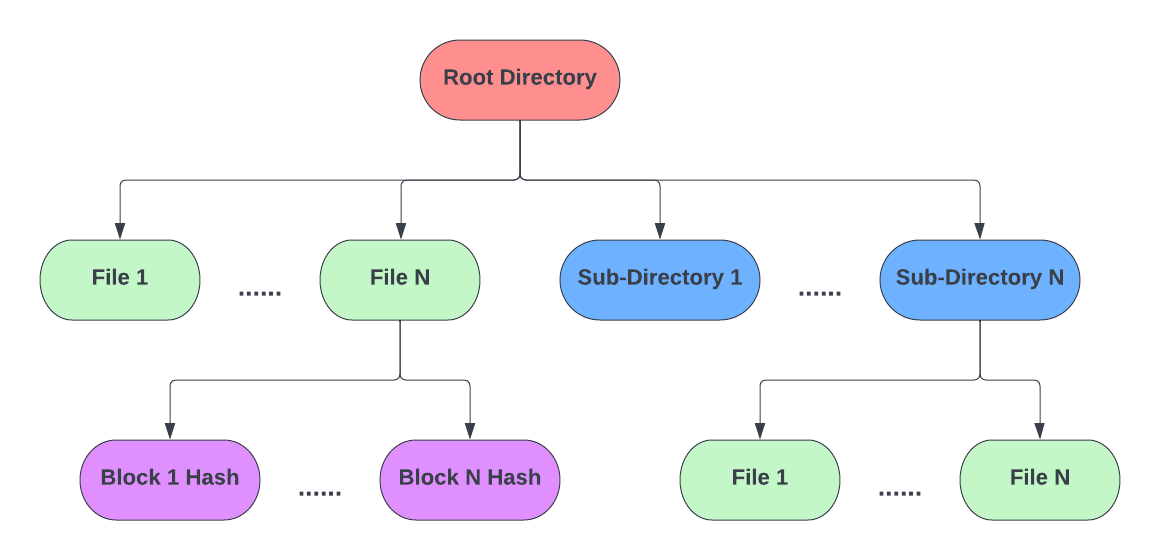
\includegraphics[width=.85\textwidth]{diagrams/block-body.png}
  \caption{\textit{How shard data is stored.}}
  \label{fig:hash-storage}
\end{figure}

\subsection{Downloading Content}

To achieve \textbf{F\_M1}, \textbf{F\_M2}, and \textbf{F\_M6}, software in the application will be content addressable and nodes will communicate with each other to collect shards. In Section~\ref{}, I mentioned how BitTorrent nodes choose, which shards of data to request first and this application will use a similar model. The general steps for downloading data are:

\begin{enumerate}
  \item A node will find the block containing information about the software they want,
  \item They send out a discover request using the root hash to find peers that are also interested in the same software and then will form connections,
  \item The node will then barter for shards of data by downloading and uploading with peers,
  \item The node will download the entirety of the software and will continue to upload it.
\end{enumerate}

\subsection{Updating Software}

As per \textbf{F\_M4}, software must be updatable through the network. To do this, when a block represents an update to a piece of software it will include the hash of the block containing the previous version of the software.

\begin{figure}[ht]
  \centering
  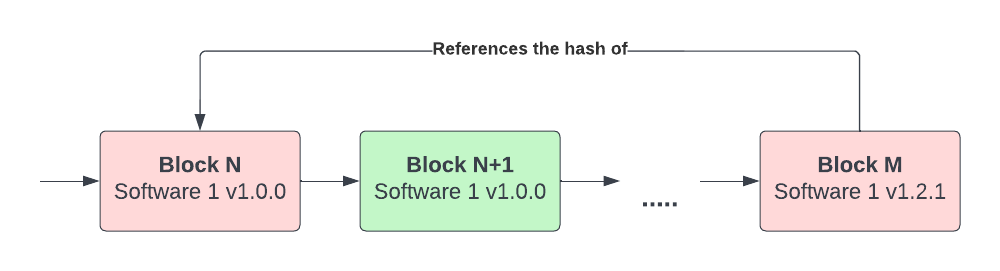
\includegraphics[width=.85\textwidth]{diagrams/update-software.png}
  \caption{\textit{How blocks can relate to older blocks.}}
\end{figure}

Each update to the software should contain its own complete directory tree, similar to Figure~\ref{fig:hash-storage}, but will likely contain duplicate hashes. When an update is released, a node will look for changes in the directory tree and request the corresponding shards. According to \textbf{F\_C1}, shards from old versions of software could be persisted but this should be down to the choice of the user.